
%----------------------------------------------------------------------------------------
%	CHAPTER 2
%----------------------------------------------------------------------------------------

\chapter{Fases del Trabajo Fin de Grado.}\label{chapter_2}

\section{Diagrama de Gantt}

En �l se puede ver de una manera general el tiempo invertido en cada una de las tareas as� como el orden en el que se han realizado. Para este trabajo se ha optado por dividirlo en dos partes. El objetivo que se sigue con ello es poder visualizarlo mejor (Figura \ref{img_gantt}). Para un mayor detalle sobre las horas dedicadas con exactitud y las acciones que se realizaron cada d�a se puede consultar el Anexo \ref{anexo:I}. 
\begin{figure}[htb]
	\centering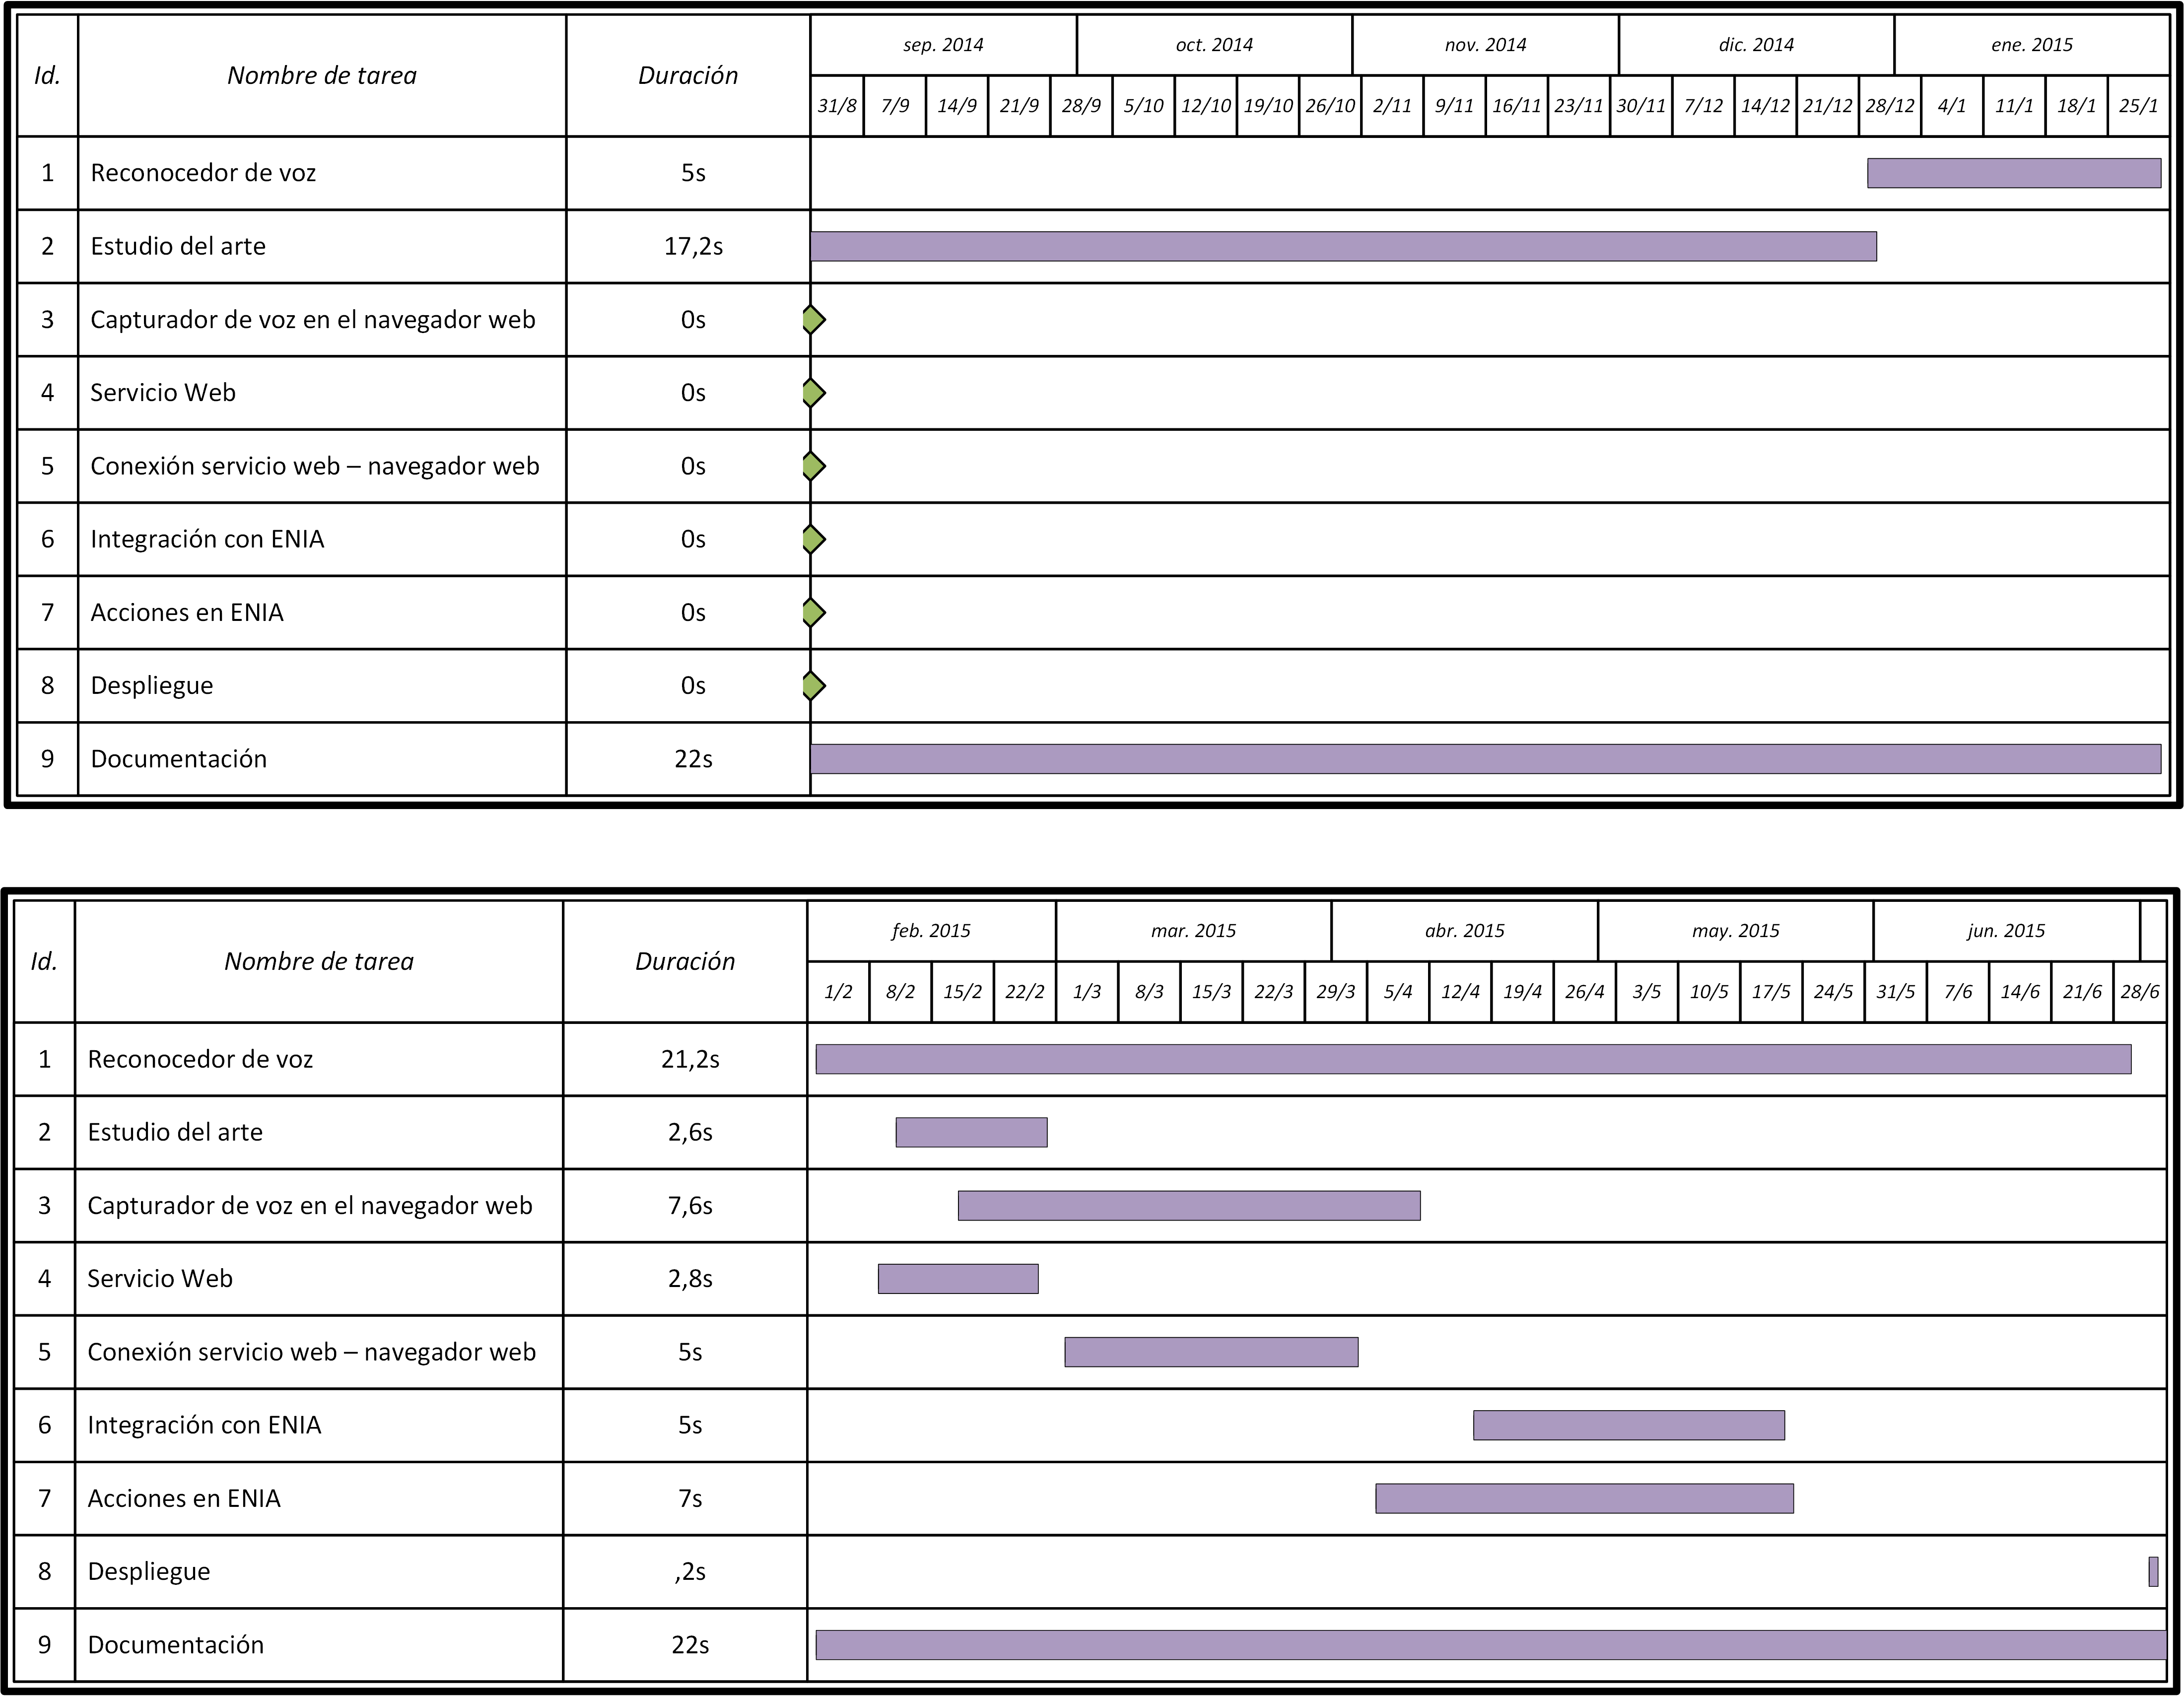
\includegraphics[scale=0.7]{DiagramaGantt}
	\caption{Diagrama de Gantt del proyecto TFG.}
	\label{img_gantt}
\end{figure}

\section{COCOMO}
% Table generated by Excel2LaTeX from sheet 'Hoja1'
\begin{table}[htbp]
	\centering
		\resizebox{\textwidth}{!} {
	\begin{tabular}{cccc}
		\toprule
		Servidor Node.js & L. implementadas & L. reutilizadas & L. autogeneradas \\
		\midrule
		package.json & 10    & 0     & 0 \\
		index.js & 76    & 0     & 0 \\
		M�dulo Ws.js & \multicolumn{3}{c}{No se ha modificado.} \\
		M�dulo socket.io & \multicolumn{3}{c}{No se ha modificado.} \\
		\midrule
		Cliente ENIA & L. implementadas & L. reutilizadas & L. autogeneradas \\
		\midrule
		index.html & 104   & 0     & 0 \\
		savins.css & 88    & 0     & 0 \\
		savins.js & 873   & 0     & 0 \\
		main.js & 0     & 211   & 0 \\
		recorder.js & 0     & 232   & 0 \\
		recorderWorker.js & 24    & 167   & 0 \\
		jquery.gridster.js & 94    & 0     & 0 \\
		\midrule
		Servicio JAX-WS & L. implementadas & L. reutilizadas & L. autogeneradas \\
		\midrule
		Transcribe.java & 15    & 0     & 0 \\
		TranscribeImpl.java & 148   & 0     & 0 \\
		enia.dict & 97    & 0     & 0 \\
		enia.gram & 28    & 0     & 0 \\
		beans.xml & 4     & 11    & 0 \\
		jboss-deployment-structure.xml & 7     & 0     & 0 \\
		web.xml & 0     & 0     & 33 \\
		pom.xml & 6     & 0     & 97 \\
		Librer�a CMU Sphinx 4 & \multicolumn{3}{c}{No se ha modificado.} \\
		&       &       &  \\
		\midrule
		Total desglosado & 1574  & 621   & 130 \\
		Total &       &       & 2325 \\
		\bottomrule
	\end{tabular}%
}
	\caption{L�neas de c�digo desglosadas por archivo.}
	\label{kloc}%
\end{table}%


A continuaci�n se va a calcular el esfuerzo persona/mes. La f�rmula es:
$$PM=A*[Size']^{B}*\prod_{i=1}^{17} EM_{i} + PM_{AT}$$

A es una constante cuyo valor es 2,5.

$Size'$ representa el n�mero de l�neas de c�digo ponderado seg�n las l�neas que se hayan desechado, desarrollado, reutilizado y autogenerado. Por tanto, $$Size' = Size * (1+\dfrac{BRAK}{100}) $$ donde \textit{BRAK} es el porcentaje de c�digo que se ha desechado. En este caso este valor es 0, por lo que queda
$$Size' = Size * (1+\dfrac{0}{100}) = Size = KNSLOC+KASLOC*\dfrac{100-AT}{100}*AAM$$ donde \textit{KNSLOC} es el n�mero de l�neas de c�digo desarrollado (en miles), es decir 1,574 \textit{KNSLOC}.
